We first analyze the results in terms of accuracy: how often the models correctly predicted whether a turn transition occurred; in other words, how often the model predicts the correct value of $y_{i+1}$.
%
Table \ref{table:result} shows the results of training a random forest of 200 trees for each model using 10 folds cross validation. We see that using the summary features provides better accuracy than baseline 1, which use only the current dialog act ($65.54\%$ vs $62.79\%$). In addition, using the full model yields an absolute improvement of over $1.08\%$ in the accuracy. In addition, baseline 1 has high precision, but very low recall. Using only the summary model improves recall and decreases precision, but leading to a higher F1 score and overall better performance. Using the full model improves precision, which means that dialog acts that were considered to lead to turn transitions are classified correctly. If we use the full model, we lose precision (over baseline 2 model), but gain recall,
leading to the highest F1 score and the best performance.
%
\begin{table}[ht!]
\begin{center}
\begin{tabular}{lrrrrr}
\toprule
{} &  Accuracy &        F1 &  Precision &    Recall &   AUC \\
\midrule
baseline 1 &  62.79\% &  57.81\% &   74.98\% &  47.04\% &  65.99\% \\
baseline 2 &  74.89\% &  74.87\% &   81.84\% &  69.00\% &  81.11\% \\
summary    &  65.54\% &  69.32\% &   67.22\% &  71.36\% &  69.46\% \\
full       &  75.75\% &  77.59\% &   77.50\% &  77.83\% &  83.78\% \\
\bottomrule
\end{tabular}
\end{center}
\caption{Precision, recall and F1 results using Random Forests }
\label{table:result}
\end{table}


The effect can also be seen in ph{was: figure}Figure \ref{auc}, which shows the ROC curves and the AUC for each
model. We notice that the AUC of the summary model is better than baseline 1 model ($0.69$ vs $0.66$), and when adding the summary features to the local features (the full model), we see the AUC improves ($0.84$ vs $0.81$). This suggests that while the discrimination facility of the summary features is lacking (AUC $<0.7$), adding them to a classifier that uses local features (full model) yields better results than the baselines.
%
 \begin{figure}[ht!]
 \centering
 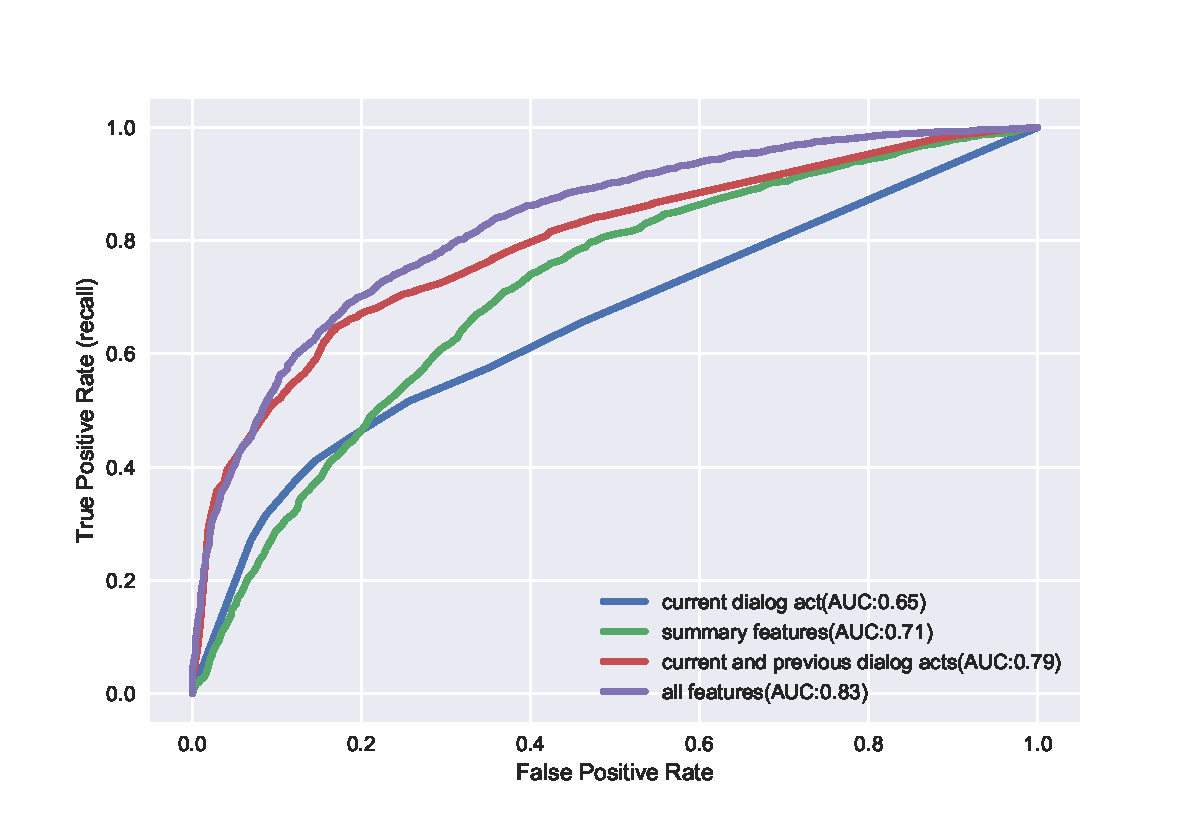
\includegraphics[width=\textwidth]{../scikitlearn/figures/roc.pdf}\vspace{-1.5em}
 \caption{ROC curves and AUC of the different models \label{overflow}}
\label{auc}
 \end{figure}

Table \ref{table:result2} shows the results of training gradient boosting classifer for each model using 10 folds cross validation. In general, the random boosting classifier perform better than random forest. Moreover, we can observe that the summary model is better than the beseline mode and the full model is better than the baseline.

\begin{table}[ht!]
\begin{center}
\begin{tabular}{lrrrrr}
\toprule
{} &  accuracy &        f1 &  precision &    recall &   roc\_auc \\
\midrule
summary    &  67.91\% &  71.30\% &   69.20\% &  73.55\% &  72.64\% \\
baseline 1 &  62.79\% &  57.81\% &   74.98\% &  47.04\% &  65.99\% \\
baseline 2 &  74.88\% &  74.82\% &   81.92\% &  68.86\% &  81.10\% \\
all        &  76.57\% &  78.74\% &   77.44\% &  80.11\% &  84.84\% \\
\bottomrule
\end{tabular}
\end{center}
\caption{Precision, recall and F1 results using Gradient boost classifier }
\label{table:result2}
\end{table}


\subsection{Sensitivity to Mesurement Start Time}

In Meshorer and Heeman \cite{Meshorer2016UsingPS}, we assumed that it take 120 seconds for the conversational image to form. So we only test our results on dialogue acts that happen more than 120 seconds into each conversation. We now evaluate this assumption by building models based on different starting times, ranging from 0s to 180s.  For the smaller start times, we also have more data, as we start analyzing the performance of our models earlier in the dialogues.  This is why the results for baseline 1 and 2 also differ with the start times.

The results are shown in Table \ref{table:starttime} in terms of the AUC scores.  As expected, we do not see much difference in the AUC values for baseline 1 and 2, so there is not much effect due to the increase in the amount of data that we are able to use.  We also do not see much difference in AUC values for the summary and full model.  This shows that the summary features predictive strength is not affected by the start time.

%
\begin{table}[ht!]
\begin{center}
\begin{tabular}{lrrrrrrr}
\toprule
{} & 0s & 15s & 30s & 45s & 60s & {\bf 120s} & 180s  \\
\midrule
baseline 1 & 65.99\% & 66.10\% & 66.12\% & 66.09\%  & 66.02\% & 65.98\% & 66.05\%  \\
baseline 2 & 81.11\% & 81.21\% & 81.24\% & 81.20\%  & 81.15\% & 80.92\% & 80.68\%  \\
summary    & 69.46\% & 69.51\% & 69.43\% & 69.49\%  & 69.57\% & 69.10\% & 69.21\%  \\
full       & 83.78\% & 83.87\% & 83.85\% & 83.80\%  & 83.61\% & 83.19\% & 82.80\%  \\

\bottomrule
\end{tabular}
\end{center}
\caption{ AUC Score in relation to the start of the dialog }
\label{table:starttime}
\end{table}



